\chapter{Introduction}
\pagenumbering{arabic}
\setcounter{page}{1}




Earth, our home planet, is the only known place in the universe that is affirmed to host life. The life on earth is characterized by three components, air, land, and water. Each element has its own special property and is required in its proper proportions to maintain the healthy life of all living beings \cite{environment}. The quality of life relies on the quality of the environment. However, industrial development and  other manmade activities create a disturbance in the natural environment. The process of making \iffalse land, water, air and other parts of the \fi environment unsuitable and unsafe for the living is called pollution. 
\par
%Pollution is a universal phenomenon that degrades the quality of environment and structures by introducing contaminant into the natural environment \cite{who}.
 Pollution changes the quality of the atmosphere and is transboundary, as they travel thousands of miles \cite{environment}. The presence of Persistent Organic Pollutants (POPs) \cite{RitterL.SolomonK.R.&Forget2005} in the environment make adverse impact on human health and sorrounding as it resist degradation by microorganisms \cite{pops}. Many types of pollution contribute to global warming and climate change which are the major issues tackled by environmental scientist these days. Out of different types of pollution, air pollution plays a major role in global warming.
 
 %are non-biodegradable and resist degradation by microorganisms; therefore they remain in the ecosystem causing adverse impact on human health and environment \cite{pops}. Global warming and related climate change are one major issues tackled by the environmental scientist.Environmental scientists these days mainly face problems related to global warming and climate change.
  
\par
 Air contamination alludes to release of pollutants into the environment that is unfavorable to human wellbeing and the planet in general. Air pollution is stated as a complex mixture of gases and particles whose sources and composition vary over space and time \cite{HealthEffectsInstitute2017}. The boom in the development of industries and technology have created an alarming situation that is, degrading the quality of air. Contamination of air is a matter of serious concern and society is quite unaware of the impact that it causes to human health as well as to the surrounding. The World Health Organization (WHO) reported that death rate estimates are around 7 million every year as 9 out of 10 people breathe polluted air \cite{who} \cite{WHO2010}. This has made many motivated individuals like researchers and communities to work towards creating awareness among the people. Various studies are underway on air pollution due to its increasing effect on the environment day by day. This brings to the reason on choosing my research topic as I always wanted to work towards a social concern. Having the background of electronics and combining with advanced computer skills seems to be a perfect combination for problem solving. In the following section, I will discuss the background to introduce my research contribution.
 
 
 
 
 %This brings to the reason why I choose to work on sensor network for air pollution and also due to my background in electronics. In the following section, I will discuss the background to introduce my research work.


\section{Air Pollutants and Measurement Metrics}


There are various pollutants that contribute to the contamination of the environment. These pollutants differ from region to region depending on the human activities. For example, an industrial area which manufactures products from raw material, such as production of iron from its ore or production of gasoline from crude oil, releases inorganic carbon compounds into the atmosphere \cite{Vallero2014}. Urban areas are the major sources of particulate matter and carbon compounds produced from the burning of fuels in the vehicle.
Based on the severity of health impact and the kind of human activities, the National Ambient Air Quality Standards (NAAQS) has set six common criteria pollutants that harm human health, environment or even property damage. The NAAQS was established by the United States Environmental Protection Agency (EPA) under the Clean Air Act which specifies the pollutants that are harmful for the public health and environment \cite{USEPA} \cite{NAAQS}. The pollutants specified by NAAQS are Particulate Matters ($PM$), Ozone ($O_3$),  Nitrogen Dioxide ($NO_2$), Carbon Monoxide ($CO$), Sulphur Dioxide ($SO_2$), and Lead ($Pb$).

Different countries measure different set of pollutants, for example, India measures 8 major pollutants such as ($PM$), ($O_3$), ($NO_2$), ($CO$), ($SO_2$), Ammonia ($NH_3$), and Benzene ($C_6H_6$) (in some places ($Pb$) instead) \cite{Chen2013}. Most other countries measures a subset of these criteria pollutant for example, Canada measures $PM$, $O_3$, $NO_2$, $SO_2$ and $CO$ \cite{Chen2013}. Particulate matters are measured at two levels; 2.5 microns size particles ($PM_{2.5}$) and 10 microns size ($PM_{10}$), and they are measured in micro-grams per cubic meters ($\mu g/m^3$). $CO$ is measured in parts per million ($ppm$) and other gases are measured in parts per billion ($ppb$). These individual measurements are not provided in layman terms and therefore are not helpful in understanding the cumulative impact of the air quality. Taking this into account the government agencies of each country around the globe developed their own indices corresponding to the NAAQS for representing the quality of air. The different indices are Air Quality Health Index (AQHI), Air Quality Index (AQI), Air Pollution Index (API), Pollution Standard Index (PSI), Comprehensive Air Quality Index (CAI), Daily Air Quality Index, Common Air Quality index (CAQI) are few used in different countries.
Out of all these indexes the most common are AQI and AQHI which are proposed and used by different countries \cite{Chen2013}.

India, USA, UK, and many other countries use AQI and Canada, Hong Kong uses AQHI. These metrics are designed  by carefully examining those pollutants which are harmful to human health and environment.
AQI is a piecewise linear function of the pollutant concentration \cite{Soni2016} and is measured using the following formula.

\begin{equation}
AQI = Max \{I_i|i = 1, ..., 8\}
\end{equation}
where $I_i$ is an air quality subindex corresponding each pollutant and it is computed as 
\begin{equation}
I_i = \lceil(\frac{I_{high} - I_{low}}{C_{high} - C_{low}})\rceil \times (C - C_{low}) + I_{low}
\end{equation}
where $C$ is concentration of the $i^{th}$ pollutant. $C_{low}$ and $C_{high}$ are lower and upper concentration breakpoints of $C$ respectively.
$I_{low}$ and $I_{high}$, respectively, are index breakpoints corresponds to $C_{low}$ and $C_{high}$.  The value of AQI varies from 0 to 400+ as shown in the Figure \ref{aqi} and each colour code shows the quality of air in the atmosphere.


\begin{figure}[h]
    \begin{center}
    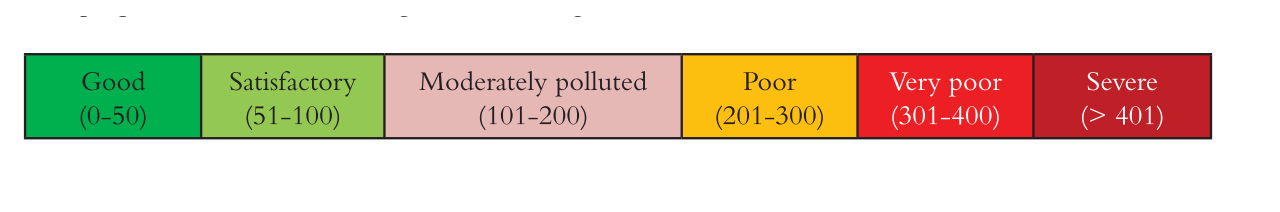
\includegraphics[scale=0.58]{./images/figure13.png}
    \end{center}
   
    \caption{Air Quality Index (AQI) \cite{AirQualityIndex}}
    
    \label{aqi}
\end{figure}


In Canada, the Environmental agency developed AQHI to make the common public aware about the quality of air that surrounds them. It was based on five major pollutants $ PM_{2.5}$, $O_3$, $NO_2$, $SO_2,$ and $CO$ initially and later the last two pollutants were dropped from the calculation as they were identified to  contribute very less in predicting health effects. AQHI is computed using the following formula.


\begin{equation}
AQHI = \lceil (\frac{1000}{10.4}) \times [e^A-1]+[e^B-1]+[e^C-1] \rceil
\end{equation}

where $ A = 0.000537 \times$ concentration of  $O_3$, $B = 0.000871 \times$ concentration  of $NO_2$ and  $C = 0.000487 \times$ concentration of $PM_{2.5}$.
The value of AQHI varies from 1 to 10+ as shown in Figure \ref{aqhi}


\begin{figure}[h]
    \begin{center}
    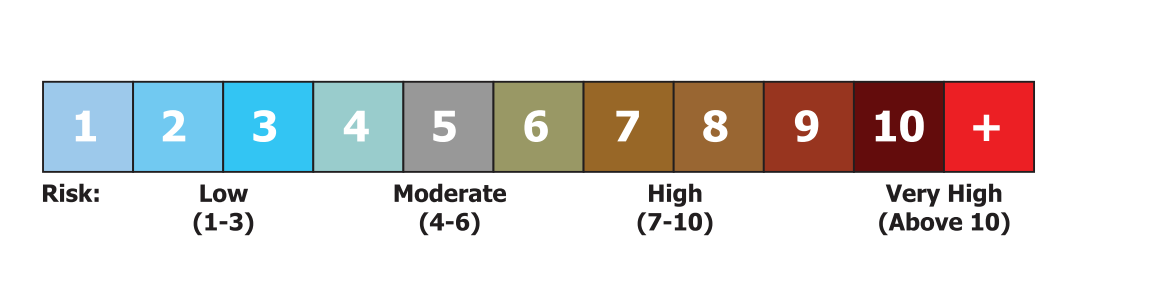
\includegraphics[scale=0.58]{./images/figure12.png}
    \end{center}
   
    \caption{Air Quality Health Index (AQHI) \cite{healthcanada}}
    
    \label{aqhi}
\end{figure}

Now the question is which is a better measure, AQI or AQHI? Health index was created with a different objective in mind that is to provide the effect of pollutants to the human health. AQI is based on a single pollutant and hence it is hard to see its direct relationship with health \cite{Chen2013}. On the other hand AQHI is based on the exposure-response relationship between the major air pollutant mix and human health \cite{Chen2013}.%which gives more close relation to the mixture of air pollutant than AQI. It is to be noted that both the indices failed to project the health outcomes associated with the exposure to the polluted environment \cite{Chen2013}. 



\section{Impact of Air Pollution}

Air pollution has significantly increased after industrialization and urbanization have taken place. The burning of fossil fuels, exhaust from factories and industries, and mining operations are major contributors towards air pollution. Exposure to air pollutants causes premature deaths, cardiovascular disease, stroke, and other respiratory diseases. The state of global air 2017 has discussed the effects of long-term exposure to harmful air pollutants such as particulate matter which contributes to over 4 million premature deaths and is estimated to double by 2050, if the issue remains unattended \cite{HealthEffectsInstitute2017}. Air pollution accounts for highest death rates annually. 

\par

Particles with a diameter of less than 10 microns ($PM_{10}$), and less than 2.5 microns ($PM_{2.5}$) causes the greatest threat to health, as they are capable of penetrating the lungs which leads to cardiovascular and Chronic Obstructive Pulmonary Diseases (COPD) \cite{who} \cite{Tian2016}. Exposure to Carbon Monoxide ($CO$) which is a colorless and odorless gas, results in absorption of the gas into bloodstream and reduces the ability of lungs to transfer oxygen which inturn affects the functionality of vital organs such as brain and the heart \cite{Sierra-vargas2012} \cite{Golbabaei2012}. Respiratory issues such as decrease in responsiveness of airways, inflammation in airways and lung infectivity occurs due to exposure of high concentration of ozone ($O_3$) \cite{Lippmann1989}. Another pollutant is nitrogen dioxide ($NO_2$) which causes illness such as wheezing, coughing, bronchitis and increases severity of flu symptoms.
\par

 The exposure of mixed air pollutants leads to health effects like birth defects, development delays in children, skin irritation or even cancer \cite{MarilenaKampa2007}. Apart from the health issues, there is a large effect in environment such as rise in sea-level, global warming that contributes to increase in overall temperature and melting of ice caps, acid rains which leads to land and crop destruction, ozone layer depletion, wildlife destruction and eutrophication which affects on aquatic life \cite{pollutioneffect}. Having discussed the effect of pollution the next section will brief about the history of air pollution and how pollution is measured. 

\section{Background}

The quality of the air has declined since the industrialization has taken place in the mid 19th century. Ever since it has affected not just the environment but also human health. Development of heavy industries across Europe and North America used coal as their major source of energy which contributed to black smoke pollution \cite{Heidorn1978} \cite{Timothy}. Coal was not just used in industries but also in houses for heating in winter which made the pollution even worse \cite{Al2016}. These emissions resulted in serious health impacts on residents in urban areas that increased the mortality rate during 19th century. 
\par
One such important event in the history of pollution is the great smog of London which killed as many as 12,000 people mostly infants. This was caused due to the combination of cold weather with smoke and lasted for several days \cite{londonfog}. There was a string of similar events reported in New York and England around the same time. All these incidents led to the development of Environmental Protection Agency (EPA) who enforced the need for installing the monitoring stations. The government along with these environmental agencies established acts like clean air act, motor vehicle air pollution act, air pollution control acts for a better quality of air\cite{airpollutionact}. Apart from that, they took initiative to monitor the air pollution by installing systems which could measure the concentration of pollutants and could give warnings to public as well as industries regarding how polluted the atmosphere is.


\subsection{Existing Environmental Monitoring station}

The government and environmental agencies are making an effort to install monitoring stations for improving the air quality. The EPA monitors the criteria pollutants along with any special pollutant that is dominant in that area. These monitoring stations are fixed in a location and are operated by environmental agencies. The stations are equipped with instruments not just monitoring criteria pollutants but also analyzes other parameters like wind speed, humidity, precipitation. These analytical instruments work by the principle of sampling of the air collected from the atmosphere.
There are two main methods for pollutant sampling: 1) passive sampling, and 2) active sampling \cite{Balakrishnan2015} \cite{activepassive}. These sampling techniques are considered as one of the most significant development for air quality measurement and  used widely for monitoring purposes. 

\par

In passive sampling the pollutants are collected by physical process such as diffusion through a static air layer or membrane. These pollutants in the air are diffused to adsorb on the sampling media due to difference in the chemical composition of pollutants. The analysis of the pollutant on the sampling media gives the time-averaged contaminant concentration \cite{Environment2009}. On the other hand, active sampling works with an air sampling pump which actively pulls the air through a collection device like filter  and weighted concentration is calculated. However these static instruments have a major drawback of temporal resolution as they are large in size and needs high maintenance. These instruments are expensive and are financially impractical to expand to more than one station. Table \ref{table:cost} gives the average estimated cost for purchasing air quality monitoring equipment produced by US Environment Protection Agency (EPA). 

\begin{table}[h]
  
  
    \begin{tabularx}{\columnwidth}{X|X}
        \hline
        Pollutant/Parameter           & Estimated cost    \\
        \hline
    
      $NOx$   & 10,4440         USD \\ 
      $SO_2$   & 35,000          USD \\ 
      $COx$   & 28,000          USD\\ 
      $Ox$   & 6,600            USD\\ 
      $PM$   & 37,700           USD\\ 
     
      FTIR Analyzer   & 100,000 USD\\ \hline
     
        
      
  \end{tabularx}
  *FTIR: Fourier Transform Infrared spectroscopy measures multiple gases 
    \caption{Estimated cost of Reference Instruments\cite{Mussatti2000}}
    \label{table:cost}
  \end{table}


As a result of high cost, only a few monitoring stations are installed for an area. Thus, we can claim that spatial resolution is limited by these conventional monitoring equipments. This made the researchers and scientists to work more on portable sensor networks to understand air pollution in a better way.


\subsection{Sensor Network for Air Quality Monitoring}

There is an emerging trend of using air sensors to understand the quality of air because of its low cost, small size and low power consumption \cite{Sun2016}. These sensors are cheaper than reference station and can be replaced easily in case of any damage. The advancement in the Micro-Electro-Mechanical System (MEMS) made it possible to integrate all the functions into a single electronic circuit which makes it more compact. These sensors do not incur deployment cost, infrastructure cost or does not require frequent maintenance which makes the overall expense even less.
\par

Sensors are used in variety of application such as military monitoring purpose, surveillance and tracking, traffic density calculation and road condition and environmental applications \cite{Kadri2013}. Sensor units can be accommodated on an automobile, building tops or even could be in a wearable form in order to track or measure. This enables high spatial resolution without establishing huge reference station \cite{Nodes2015}. Sensors measuring different compounds are integrated together to make a sensor node system. Extensive research works have been done with the available sensors in the market.

\section{Motivation}

One of the important components in solving the issue of air pollution is to increase the awareness among public about the current situation and its impact so that they can act on it. The conventional method of monitoring the air quality with the help of a few heavyweight expensive stationary monitoring systems typically installed by the state may not be effective enough for this task. To achieve the goal effectively and without further delay, pollution monitoring must become part of daily activity for everyone. For that, the devices to monitor pollution must be small, portable, inexpensive, and part of a global system. With the technological advancement of low-cost computing, communication, and sensing devices, and the revolution of open source software \cite{Anthes2016}, we believe it is possible to build pervasive air pollution monitoring system with the available sensors from the market and building an open source software. Now the question is how to design such pollution monitoring devices faster and make them accessible to as many people as possible. 

\par

Achieving the above stated goal requires a suitable system framework that can help to accelerate the process of the design and implementation of an air pollution monitoring system using the off-the-shelf hardware and building an open source tool for representing the collected data from sensor. Some recent attempts to build a low cost air pollution monitoring system have been done, however, none of them are simple and easily re-producable. This thesis is an attempt to fill that gap by first proposing a simple and comprehensive framework and then demonstrating its feasibility and use by creating our own low cost and easy to use pollution monitoring system that is operational in our lab. We have also added a step of calibration by implementing a web-based tool to ensure that we measure high quality data. Our contribution is a step towards inspiring and motivating not only the public to use the device, but also many amateur electronic hobbyists to buy the hardware locally and download the associated software to build their own pollution monitoring device.


\section{Research Problem}

This thesis focuses on design and development of an air pollution monitoring system using off-the-shelf
hardware and build an open source software that focuses on three different types of users with the following objectives in mind:
\begin{enumerate}
  \item To demonstrate the quality of data obtained from the low cost system by comparing it with the expensive monitors fixed at a particular location.
  
  \item To encourage citizen to contribute in solving the issue of air pollution and to give more insight about the impact it causes to human health and environment.
   
  \item To give an idea on how to integrate the hardware components to a processor and also make an independent software, which can be accessed world-wide.
  
  \item To provide user oriented data which gives a deeper understanding about the pollution.
  
  \item To provide information on the quality of air by including Air Quality Health Index (AQHI) which provides a measure of adverse affects on health by pollutants and Air Quality Index (AQI) that gives an idea about the level of pollution on the environment.

  
  \item Improving the quality of data obtained from the system by integrating a calibration tool.
  

   

\end{enumerate}


\section{Thesis Contribution}

There are three major contribution from thesis:
\begin{enumerate}
  
    \item Air pollution monitoring system: The system itself which measures the pollutants from the atmosphere. This include the sensors with the processor and the data trasferring module. We believe that this could be a way to show that low cost system could be used for data collection.
    
    \item  Air pollution visualization software: Next major contribution is the the software that could be used for data visualization. The main idea is to make the collected data user sensitive and hence we came up with the idea of building the complete tool from the scratch as the already available tools in the market are paid service. 
    
    \item Integration of Calibration tool :  Macro Analysis Tool (MAT) developed by Environmental Protection Agency (EPA)\cite{airsensorguidebook} which is an excel based tool was modified into a web-based tool which provides an access for any user to understand the quality of data obtained.
  
\end{enumerate}


\section{Research Question}
 
 Some important research questions to be addressed related to the issue of air quality are: 

 \begin{enumerate}
 
  \item What kind pollutants affect the human health most? How to measure them?
   
  \item  As the pollution is in the atmosphere, should it not be measured everywhere all the time? If so, what kind of infrastructure is needed to facilitate such a ubiquitous measurement?
  
 \item What all factors should be considered while selecting sensors for measurement of pollutants?
 
 \item Which processor to be used for processing the data collected from sensors?
 
 \item How should the hardware component i.e the sensors and the processor, should be packaged?
 
 \item What is the difference between different metrics which is used to show       	the effect of pollution?

\item How can the seriousness of pollution be made aware?

 \item How can the representation of Air quality metrics be done?
 
 \end{enumerate}
 
\section{Research Challenges}


The major challenges experienced on creating a complete system are:

\begin{enumerate}


\item The integration of different sensors with the processor.
\par
As each sensor has its own property, there can be issues when connecting all of them together in a single platform. Most of the sensors used for measurement are heat sensor and needs to be powered atleast 12 hours before operating. There is a particular operating temperature range for each sensor  connected. As each of the sensor needs different environment for working, all the factors should be incorporated for a complete working environment.



\item Calibration of each sensors based on the data sheet.
\par
As I am selecting low cost sensors which comes with calibration with respect to the environment it was developed. The collected data changes for each environment and this should be taken care of. This can be a tough task as for each of the sensors it changes based on the slope of internal resistance and the internal voltage values given in data sheet. 


\item Packaging of hardware component.
\par
To make the whole system portable it should be packed carefully. For certain sensor like dust sensor, it should be exposed to the environment so as to estimate the particulate matter. This packing should be done in such a way that the it does not hinder with the observed value.

\item Development of the visualization software.
\par The development of user specific visualization tool from the scratch was most challenging as this was my first hands on experience in creating a tool which involved different methods of data display. Another task was to make the tool connect to the backend python code which does the data clensing and calibration which took a lot of preparation work.

\item Transferring the data to a platform or a database using the WiFi module.

\item Checking whether the collected data is accurate.


\end{enumerate}

\section{Structure of the Thesis}

Rest of the thesis is organized as follows. Chapter 2 focuses on related work for different methods of understanding and detecting pollution. This is divided into four main categories and  work done in each category is explained further. Next, in Chapeter 3 the design and implementation of pollution monitoring system and the visualization tool is explained. To test the accuracy of collected data to the orginal data we have implemented calibration tool by linear regression which is described in Chpater 4. In Chapter 5, analysis of the results obtained from the system is demonstrated. Finally, in Chapter 6 the conclusion and direction for future work are provided.